\documentclass[
  captions=tableheading,
  bibliography=totoc, 
  titepage=firstiscover,
]{scrartcl}

\usepackage{blindtext} %neuer input

\usepackage{longtable} % Tabellen über mehrere Seiten

\usepackage[utf8]{inputenc} %neuer input

\usepackage{scrhack}

\usepackage[aux]{rerunfilecheck} %Warnung falls nochmal kompiliert werden muss

\usepackage{fontspec} %Fonteinstellungen

\recalctypearea{}

\usepackage[main=ngerman]{babel} %deutsche Spracheinstellung

\usepackage{ragged2e} %neuer input

\usepackage{amsmath, nccmath}

\usepackage{amssymb} %viele mathe Symbole

\usepackage{mathtools} %Erweiterungen für amsmath


\DeclarePairedDelimiter{\abs}{\lvert}{\rvert}
\DeclarePairedDelimiter{\norm}{\lVert}{\rVert}

\DeclarePairedDelimiter{\bra}{\langle}{\rvert}
\DeclarePairedDelimiter{\ket}{\lvert}{\rangle}

\DeclarePairedDelimiterX{\braket}[2]{\langle}{\rangle}{
#1 \delimsize| #2
}

\NewDocumentCommand \dif {m}
{
\mathinner{\symup{d} #1}
}


\usepackage[
  math-style=ISO,
  bold-style=ISO,
  sans-style=italic,
  nabla=upright,
  partial=upright,
  warnings-off={
    mathtools-colon,
    mathtools-overbracket,
  },
]{unicode-math}

\setmathfont{Latin Modern Math}
\setmathfont{XITS Math}[range={scr, bfscr}]
\setmathfont{XITS Math}[range={cal, bfcal}, StylisticSet=1]


\usepackage[
  locale=DE,
  separate-uncertainty=true,
  per-mode=reciprocal,
  output-decimal-marker={,},
]{siunitx}

\usepackage[autostyle]{csquotes} %richtige Anführungszeichen

\usepackage{xfrac}

\usepackage{float}

\floatplacement{figure}{htbp}

\floatplacement{table}{htbp}

\usepackage[ %floats innerhalb einer section halten
  section,   %floats innerhalb er section halten
  below,     %unterhalb der Section aber auf der selben Seite ist ok
]{placeins}

\usepackage[
  labelfont=bf,
  font=small,
  width=0.9\textwidth,
]{caption}

\usepackage{subcaption} %subfigure, subtable, subref

\usepackage{graphicx}

\usepackage{grffile}

\usepackage{booktabs}

\usepackage{microtype} %Verbesserungen am Schriftbild

\usepackage[
backend=biber,
]{biblatex}

\addbibresource{../lit.bib}

\usepackage[ %Hyperlinks im Dokument
  german,
  unicode,
  pdfusetitle,
  pdfcreator={},
  pdfproducer={},
]{hyperref}

\usepackage{bookmark}

\usepackage[shortcuts]{extdash}

%\usepackage{warpcol}


\begin{document}
    \title{V101 Das Trägheitsmoment}
    \author{  
    Tobias Rücker\\
    \texorpdfstring{\href{mailto:tobias.ruecker@tu-dortmund.de}{tobias.ruecker@tu-dortmund.de}
    \and}{,} 
    Paul Störbrock\\
    \texorpdfstring{\href{mailto:paul.stoerbrock@tu-dortmund.de}{paul.stoerbrock@tu-dortmund.de}}{}
    }
    \date{Durchführung: 03.12.2019, Abgabe: 10.12.2019\vspace{-4ex}}
\maketitle
\center{\Large Versuchsgruppe: \textbf{42}}
    
    \begin{abstract}
    \centering
        \textbf{Ziel:} Messung des Trägheitsmoments verschiedener Körper und Nachweis des Satzes von Steiner
    \end{abstract}

\newpage
\tableofcontents
\newpage

% Theorie %%%%%%%%%%%%%%%%%%%%%%%%%%%%%%%%%%%%%%%%%%%%%%%%%%%%%%%%%%%%%%%%%%%%%%%%%%%%%%%%%%%%%%%%%%%%%%%%%
\section{Theorie}\justifying
\begin{align}
    \intertext{Rotationsbewegungen beschreiben Bewegungen bei denen sich eine Massenverteilung
    um eine Rotationsachse dreht. Dabei werden diese Bewegungen hauptsächlich durch die Größen
    beschrieben: dem Trägheitsmoment $I$, dem Drehmoment $M$ und der Winkelbeschleunigung $\dot{\omega}$.
    Das Trägheitsmoment beschreibt dabei eine skalare Größe, welche ein Maß der Trägheit einer Massenverteilung
    gegenüber Rotationen darstellen. Es bildet damit ein Äquivalent zur Masse in Translationsbewegungen.
    Ein Trägheitsmoment hängt dabei explizit von dem Abstand zur und der Wahl der Rotationsachse ab.
    Für eine Punktmasse zum Beispiel, lässt sich das Trägheitsmoment durch folgende Formel 
    beschreiben \cite{V101}:
    }
    I &= m  r^2 \label{eq:1}
    \intertext{Für ausgedehnte Massekörper wird diese Formel über infinitesimal kleine Massestücke aufintegriert \cite{V101}:
    }
    I &= \int r^2 \symup{d} \, m \label{eq:2}
    \intertext{Für homogene Körper lassen sich diese Integrale einfach lösen. 
    Einige Beispiele für Trägheitsmomente einfacher Körper sind das Trägheitsmoment einer homogenen Vollkugel durch seinen 
    Mittelpunkt \cite{V101}:
    }
    I_{\text{Kugel}} &= \frac{2}{5} m R^2 \label{eq:3}
    \intertext{Das Trägheitsmoment eines homogenen Vollzylinders mit der Drillachse durch den  Mittelpunkt des Bodens \cite{V101}:
    }
    I_{\text{Zylinder,v}} &= \frac{mR^2}{2} \label{eq:4}
    \intertext{Und das Trägheitsmoment eines homogenen Vollzylinders deren Drillachse senkrecht zum Mantel durch den
    Schwerpunkt verläuft \cite{V101}:
    }
    I_{\text{Zylinder,h}} &= m \left( \frac{R^2}{4}+\frac{h^2}{12} \right) \label{eq:5}
    \intertext{Bei komplexeren Körper wird versucht den Schwerpunkt durch eine Zusammensetzung einfacher Körper zu beschreiben.
    Verläuft die Drillachse parallel zu einer Achse durch den Schwerpunkt, wird das Trägheitsmoment
    mithilfe des Steinerschen Satzes berechnet \cite{V101}:
    \newline
    }
    I &= I_s+m \cdot a^2 \label{eq:6}
    \intertext{$I_s$ beschreibt dabei das Trägheitsmoment bezüglich der parallelen Drillachse durch den Schwerpunkt.
    Die skalare Größe $a$ stellt dabei den Abstand der beiden parallelen Achsen dar.
    Das Drehmoment ist definiert als die Kraft, welche an einen drehenden Körper ansetzt.
    Beschreiben lässt sich dieser durch \cite{V101}:
    \newline
    }
    \vec{M} &= \vec{F} \times \vec{r} \label{eq:7}
    \intertext{Liegt nun ein oszillierendes System vor, welches um einen Winkel $\varphi$
    ausgelenkt wird, so wirkt der Feder eine rücktreibende Kraft der Bewegung entgegen.
    Die Periodendauer der Schwingung kann dabei beschrieben werden durch \cite{V101}:
    }
    T &= 2 \pi \sqrt{\frac{I}{D}} \label{eq:8}
    \intertext{Wobei das Dremoment $M$ und die Winkelrichtgröße $D$ in folgender Beziehung
    stehen \cite{V101}:
    }
    M &= D \cdot \varphi \label{eq:9}
\end{align}

% Fehlerrechnung %%%%%%%%%%%%%%%%%%%%%%%%%%%%%%%%%%%%%%%%%%%%%%%%%%%%%%%%%%%%%%%%%%%%%%%%%%%%%%%%%%%%%%%%%%%%%%%%%%%
\section{Fehlerrechnung}\justifying
Für die Auswertung werden im folgenden diese Formeln zur Bestimmung der Fehler verwendet:
\begin{subequations}
\begin{align}
\intertext{Der Mittelwert wird berechnet mit:
}
    \overline{x} &= \frac{1}{N}\sum_{i=1}^{N} x_i \label{eq:10a}.
\intertext{Der Fehler des Mittelwerts wird berechnet:
}
    \Delta\overline{x} &= \frac{1}{\sqrt{N}} \sqrt{\frac{1}{1-N} \sum_{i=1}^{N} (x_i - \overline{x})^2} \label{eq:10b},
\intertext{Und die Gaußsche Fehlerfortpflanzung wird mit der folgenden Formel berechnet:
}
    \Delta f &= \sqrt{\sum_{i=1}^{N} \left( \frac{\delta f}{\delta x_i} \right)^2 \cdot (\Delta x_i)^2} \label{eq:10c}
\intertext{Zur Berechnung von Ausgleichsgeraden werden dabei}
        y &= m \cdot x + b \label{eq:10d} \\ 
        m &= \frac{\overline{xy} - \overline{x} \cdot \overline{y}}{\overline{x^2} - {\overline{x}}^2} \label{eq:10e}\\
        b &= \frac{\overline{y} \cdot \overline{x^2} - \overline{xy} \cdot \overline{x}}{\overline{x^2} - {\overline{x}}^2} \label{eq:10f}
\end{align}
\end{subequations}


% Versuchsaufbau %%%%%%%%%%%%%%%%%%%%%%%%%%%%%%%%%%%%%%%%%%%%%%%%%%%%%%%%%%%%%%%%%%%%%%%%%%%%%%%%%%%%%%%%%%%%%%%%%%%%%%%%%%%%%%%%%%%%%%%%%%%%%%%%%%%%%%%%%%%
\section{Versuchsaufbau}\justifying

Benötigt werden: \textit{Eine Drillachse die durch eine Spiralfeder mit einem festen Rahmen verbunden ist, eine Stabachse der Länge $\SI{62}{\centi\meter}$, 
zwei identische zylindrische Gewichte ($\SI{261.5}{\gram}$), eine Kugel mit Aufsatz (m=$\SI{1168.5}{\gram}$, r=$\SI{7.3}{\centi\meter}$), einen Zylinder mit 
Aufsatz (m=$\SI{1525.5}{\gram}$, h=$\SI{13,95}{\centi\meter}$, d=$\SI{8}{\centi\meter}$), eine Holzpuppe mit Aufsatz ($\rho=\SI{780}{\kilo\gram\per\cubic\meter}$), 
ein Newtonmeter (von $\SI{0.1}{\newton}$ bis $\SI{1}{\newton}$), eine Drehwinkel-Messscheibe, ein Ma\ss band, eine Schieblehre, eine Stopuhr.}\\
Zu Beginn wird die Stabachse horizontal auf der Drillachse befestigt. An beiden Enden der Stabachse werden die beiden zylindrischen Gewichte angebracht.
Anschließend wird die Kugel auf die Drillachse gesteckt.
Der Zylinder wird längs auf der Drillachse aufgesteckt. 
Zum Schluss wird die Puppe in einer stehenden Position, einmal mit angelegten Armen und einmal mit ausgestreckten, senkrecht zum Körper befindlichen
Armen, auf der Drillachse befestigt.

% Versuchsdurchführung %%%%%%%%%%%%%%%%%%%%%%%%%%%%%%%%%%%%%%%%%%%%%%%%%%%%%%%%%%%%%%%%%%%%%%%%%%%%%%%%%%%%%%%%%%%%%%%%%%%%%%%%%%%%%%%%%%%%%%%%%%%%%%%%%%%%%%%%%%%
\section{Versuchsdurchführung}\justifying

Um die Trägheitsmomente der einzelnen Körper zu berechnen, soll zuerst das Trägheitsmoment der Drillachse bestimmt werden. Infolgedessen wird die
Stabachse auf der Drillachse befestigt. Die beiden zylindrischen Gewichte werden mit einem Abstand von $\SI{25}{\centi\meter}$ zur Mitte an beiden 
Enden der Stabachse angebracht. Daraufhin wird die Stabachse um einen konstanten Winkel $\varphi = \SI{20}{\degree}$ ausgelenkt und die Periodendauer mithilfe
einer Stoppuhr über drei Perioden genau zweimal gemessen. Dies wird für jede Reduzierung des Abstandes um $\SI{2.5}{\centi\meter}$ wiederholt, bis beide 
Massen bei einem Abstand von $\SI{2.5}{\centi\meter}$ zur Mitte angekommen sind.\\
Neben dem Trägheitsmoment der Drillachse ist die Federkonstante der Spiralfeder für die folgenden Trägheitsmomente wichtig. Um diese zu bestimmen 
werden die Massen von der Stabachse genommen und diese um einen Winkel von $\SI{90}{\degree}$  ausgelenkt. Nun wird das Newtonmeter an einem konstanten Abstand von 
$\SI{30}{\centi\meter}$ zur Mitte angesetzt und die Kraft der Spiralfeder übers Newtonmeter aufgenommen. Dabei wird das Newtonmeter
senkrecht zum Radius der Kreisbahn gehalten. Anschließend werden die Kräfte für eine schrittweise Erhöhung des Auslenkwinkels um $\SI{10}{\degree}$ gemessen,
bis der ein Wert von $\SI{260}{\degree}$ erreicht wird.\\
Nachdem Federkonstante und Trägheitsmoment der Drillachse bestimmt wurden, können die Trägheitsmomente des Zylinders, der Kugel und der Puppe
errechnet werden. Für die Kugel werden fünf Werte für die Schwingdauer einer Periode $T$ bei einem konstanten Winkel von $\SI{20}{\degree}$ erfasst.
Für den Zylinder werden ebenfalls fünf Messwerte für eine Periode aufgenommen, bei einem konstanten Winkel von $\SI{10}{\degree}$. 
Zuletzt werden die Schwingperioden der Puppe in Position 1 (Arme angelegt) und Position 2 (Arme ausgestreckt) gemessen. Dafür wurde der Auslenkwinkel
bei $\SI{10}{\degree}$ konstant gehalten. Um bei einer kurzen Schwingdauer verlässliche Messwerte zu erhalten, wurde die Zeitlupenfunktion einer 
Handykamera verwendet. Das Video zeigt die Schwingung der Puppe und die Stopuhr, welche den zeitlichen Verlauf der Schwingung verdeutlicht.\\
\newpage
% Auswertung %%%%%%%%%%%%%%%%%%%%%%%%%%%%%%%%%%%%%%%%%%%%%%%%%%%%%%%%%%%%%%%%%%%%%%%%%%%%%%%%%%%%%%%%%%%%%%%%%%%%%%%%%%%%%%%%%%%%%%%%%%%%%%%%%%%%%%%%%%%
\section{Auswertung}\justifying
\subsection{Maße der einzelnen Körper}
\label{sec:6.1}
\flushleft
\begin{align*}
\intertext{Zylinder:}
    &\text{Durchmesser:} &\SI{8}{\centi\meter}\\
    &\text{Höhe:}  &\SI{30}{\centi\meter}\\
    &\text{Gewicht:} &\SI{1525.5}{\gram} 
\intertext{Kugel:}
    &\text{Durchmesser:} &\SI{14.6}{\centi\meter}\\
    &\text{Gewicht:} &\SI{1168.5}{\gram}
\intertext{Puppe (Kopf):}
    &\text{Durchmesser:} &\SI{3.265}{\centi\meter}\\
    &\text{Höhe:}  &\SI{4.380}{\centi\meter}\\
    &\text{Gewicht:} &\SI{28.60}{\gram} 
\intertext{Puppe (Torso):}
    &\text{Durchmesser:} &\SI{3.89}{\centi\meter}\\
    &\text{Höhe:}  &\SI{9.625}{\centi\meter}\\
    &\text{Gewicht:} &\SI{89.22}{\gram} 
\intertext{Puppe (Arm):}
    &\text{Durchmesser:} &\SI{1.65}{\centi\meter}\\
    &\text{Höhe:}  &\SI{13.25}{\centi\meter}\\
    &\text{Gewicht:} &\SI{22.10}{\gram} 
\intertext{Puppe (Bein):}
    &\text{Durchmesser:} &\SI{2.18}{\centi\meter}\\
    &\text{Höhe:}  &\SI{14.475}{\centi\meter}\\
    &\text{Gewicht:} &\SI{42.14}{\gram} 
\end{align*}

\subsection{Die Drillachse}\justifying % Drillachse ---------------------------------------------------------------------------------------------------------

\begin{align}
\intertext{\flushleft{Um\;}\justifying das Trägheitsmoment der Drillachse zu bestimmen wird die Formel \eqref{eq:8} nach I umgestellt und mit Formel % Trägheitsmoment I_D ---------------------------------------------------------------------------------------------------------
\eqref{eq:6} gleichgesetzt. Die resultierende Gleichung sieht aus wie folgt:
}
T^2 = I_S \cdot \frac{4\pi^2}{D} &+ \frac{m_k \cdot 4\pi^2}{D} \cdot a^2 \label{eq:11}
\intertext{Hierbei wird festgestellt, dass
}
b &= I_S \cdot \frac{4\pi^2}{D} \label{eq:12}
\intertext{entspricht.
Daraus folgt für das Trägheitsmoment der Drillachse:
}
I_D &= \frac{b \cdot D}{4 \pi^2} \label{eq:13}
\end{align}

\begin{table}[H]
    \centering
    \input{table_IStab.tex}
    \caption{Tabelle der Messwerte für das Trägheitsmoment der Stabachse $I_D$}
    \label{tab:1}
\end{table}

\flushleft{Für} die Berechnung wurden zwei Werte der Periodendauer für einen Abstand gemessen und in der Tabelle \ref{tab:1}
zusammengetragen. Diese zwei Werte wurden gemittelt und auf eine Periode normiert.

\flushleft{Mithilfe\;}\justifying der Formel \eqref{eq:12} und dem Pyton Befehl linregress() \cite{numpy} lässt sich die Geradengleichung
des folgenden Graphen \ref{fig:1} bestimmen. 
\flushleft{Dabei\;}\justifying sehen die Steigung $m$ und der Schnittpunkt der y-Achse $b$ des Graphen \ref{fig:1} folgendermaßen aus:

\begin{subequations}
\begin{align}
m &= \text{\input{slope.tex}}\label{eq:14a}\\
b &= \text{\input{intercept.tex}}\label{eq:14b}
\end{align}
\end{subequations}

\begin{figure}[H]
    \centering
    \includegraphics[width=0.75\textwidth]{plot.pdf}
    \caption{Lineare Regression für $I_{Stab}$}
    \label{fig:1}
\end{figure}


\flushleft{Aus\;}\justifying der linearen Regression lässt sich das Trägheitsmoment der Drillachse mit Formel \eqref{eq:13} bestimmten:
\begin{equation}
I_D = \input{I_D.tex}\label{eq:15} % Trägheitsmoment Drillachse
\end{equation}

% Federkonstante --------------------------------------------------------------------------------------------------------------------------

\flushleft{Für\;}\justifying die Winkelrichtgröße wurde die Formel \eqref{eq:7} mit der Formel \eqref{eq:9} gleichgesetzt. Formel \eqref{eq:7} kann durch $M = \abs{\vec{F}} \cdot \abs{\vec{r}}$
dargestellt werden, da die Kraft der rücktreibenden Kraft senkrecht zum Radius steht. Wird die gewonnene Gleichung nach $D$ umgestellt, folgt:
\begin{equation}
D = \frac{F\cdot r}{\varphi}\label{eq:16}
\end{equation}

\begin{table}[H]
    \centering
    \input{table_D.tex}
    \caption{Tabelle der Messwerte für die Winkelrichtgröße $D$}
    \label{tab:2}
\end{table}


\flushleft{Die\;}\justifying Winkelrichtgröße der Spiralfeder berechnet sich aus dem Mittelwert \eqref{eq:10a} der einzelnen Winkelrichtgrößen aus 
Formel \eqref{eq:12} mit den Werten aus Tabelle \ref{tab:2} und ergibt:

\begin{equation}
\overline{D} = \text{\input{D_mean.tex}} \label{eq:17} % Federkonstante der Spiralfeder
\end{equation}

\flushleft{Um} im folgenden für verschiedene Körper mithilfe der Formel \eqref{eq:11} das Trägheitsmoment
berechnen zu können, muss bedacht werden, dass sich das Trägheitsmoment im Schwerpunkt 
aus $I_D$ und dem Trägheitsmoment des Körpers $I_K$ zusammensetzt. Dadurch ergibt sich 
für $I_K$:
\begin{align}
    I_K = \frac{T^2 \cdot D}{4 \pi^2}-ma^2-I_D\label{eq:18}
\end{align}

\subsection{Der Zylinder}\justifying % Zylinder ---------------------------------------------------------------------------------------------------------

\begin{table}[H]
    \centering
    \input{table_I.tex}
    \caption{Tabelle der Messwerte für die Perioden $T$ der einzelnen Körper}
    \label{tab:3}
\end{table}

\begin{subequations}
\begin{align}
\intertext{\flushleft{Für\;}\justifying den experimentellen Wert des Trägheitsmoments des Zylinders wurde die Formel \eqref{eq:11} nach $I_S$ umgestellt.
Die Werte für die Periodendauer aus der Tabelle \ref{tab:3} wurden für alle folgenden Berechnungen auf eine Nachkommastelle gerundet.
Daraus folgt das errechnete Trägheitsmoment des Zylinders mit den Werten aus Tabelle \ref{tab:3} und einer Masse von $\SI{1525.5}{\gram}$:
}
I_{Zy, exp.} &= \input{I_Zylinder_mean.tex}\label{eq:19a}
\intertext{\flushleft{Das\;}\justifying theoretische Trägheitsmoment des Zylinders wurde mit der Formel \eqref{eq:5} und den Werten für $T$ aus Tabelle 
\ref{tab:3} bestimmt und lautet:
\newline
}
I_{Zy, lit.} &= \input{I_Zylinder_Theorie.tex}\label{eq:19b}
\intertext{\flushleft{Der\;}\justifying daraus resultierende relative Fehler des Trägheitsmoments vom Zylinder beträgt:
\newline
}
\frac{I_{Zy, exp.} - I_{Zy, lit.}}{I_{Zy, lit.}} &= \input{RF_I_Zylinder.tex}\label{eq:19c}
\end{align}
\end{subequations}

\subsection{Die Kugel}\justifying % Kugel ---------------------------------------------------------------------------------------------------------

\flushleft{Das\;}\justifying experimentelle Trägheitsmoment der Kugel wurde mit der selben Formel \eqref{eq:11} bestimmt, wie das des Zylinders.
Die Werte für $T$ werden der Tabelle \ref{tab:3} entnommen. 
Demnach lautet der experimentelle Wert des Trägheitsmoments:
\begin{subequations}
\begin{align}
I_{Ku, exp.} &= \input{I_Kugel_mean.tex} \label{eq:20a}
\intertext{\flushleft{Das\;}\justifying theoretische Trägheitsmoment der Kugel wurde mit der Formel \eqref{eq:3} und den Werten 
aus Tabelle \ref{tab:3} bestimmt:
}
I_{Ku, lit.} &= \input{I_Kugel_Theorie.tex} \label{eq:20b}
\intertext{\flushleft{Der\;}\justifying relative Fehler des Trägheitsmoments der Kugel ist:
}
\frac{I_{Ku, exp.} - I_{Ku, lit.}}{I_{Ku, lit.}} &= \input{RF_I_Kugel.tex} \label{eq:20c}
\end{align}
\end{subequations}

\subsection{Puppe}\justifying % Puppe ---------------------------------------------------------------------------------------------------------
\begin{figure}[H]
\caption{Positionen der Puppe}
\begin{subfigure}{0.495\linewidth}
\centering
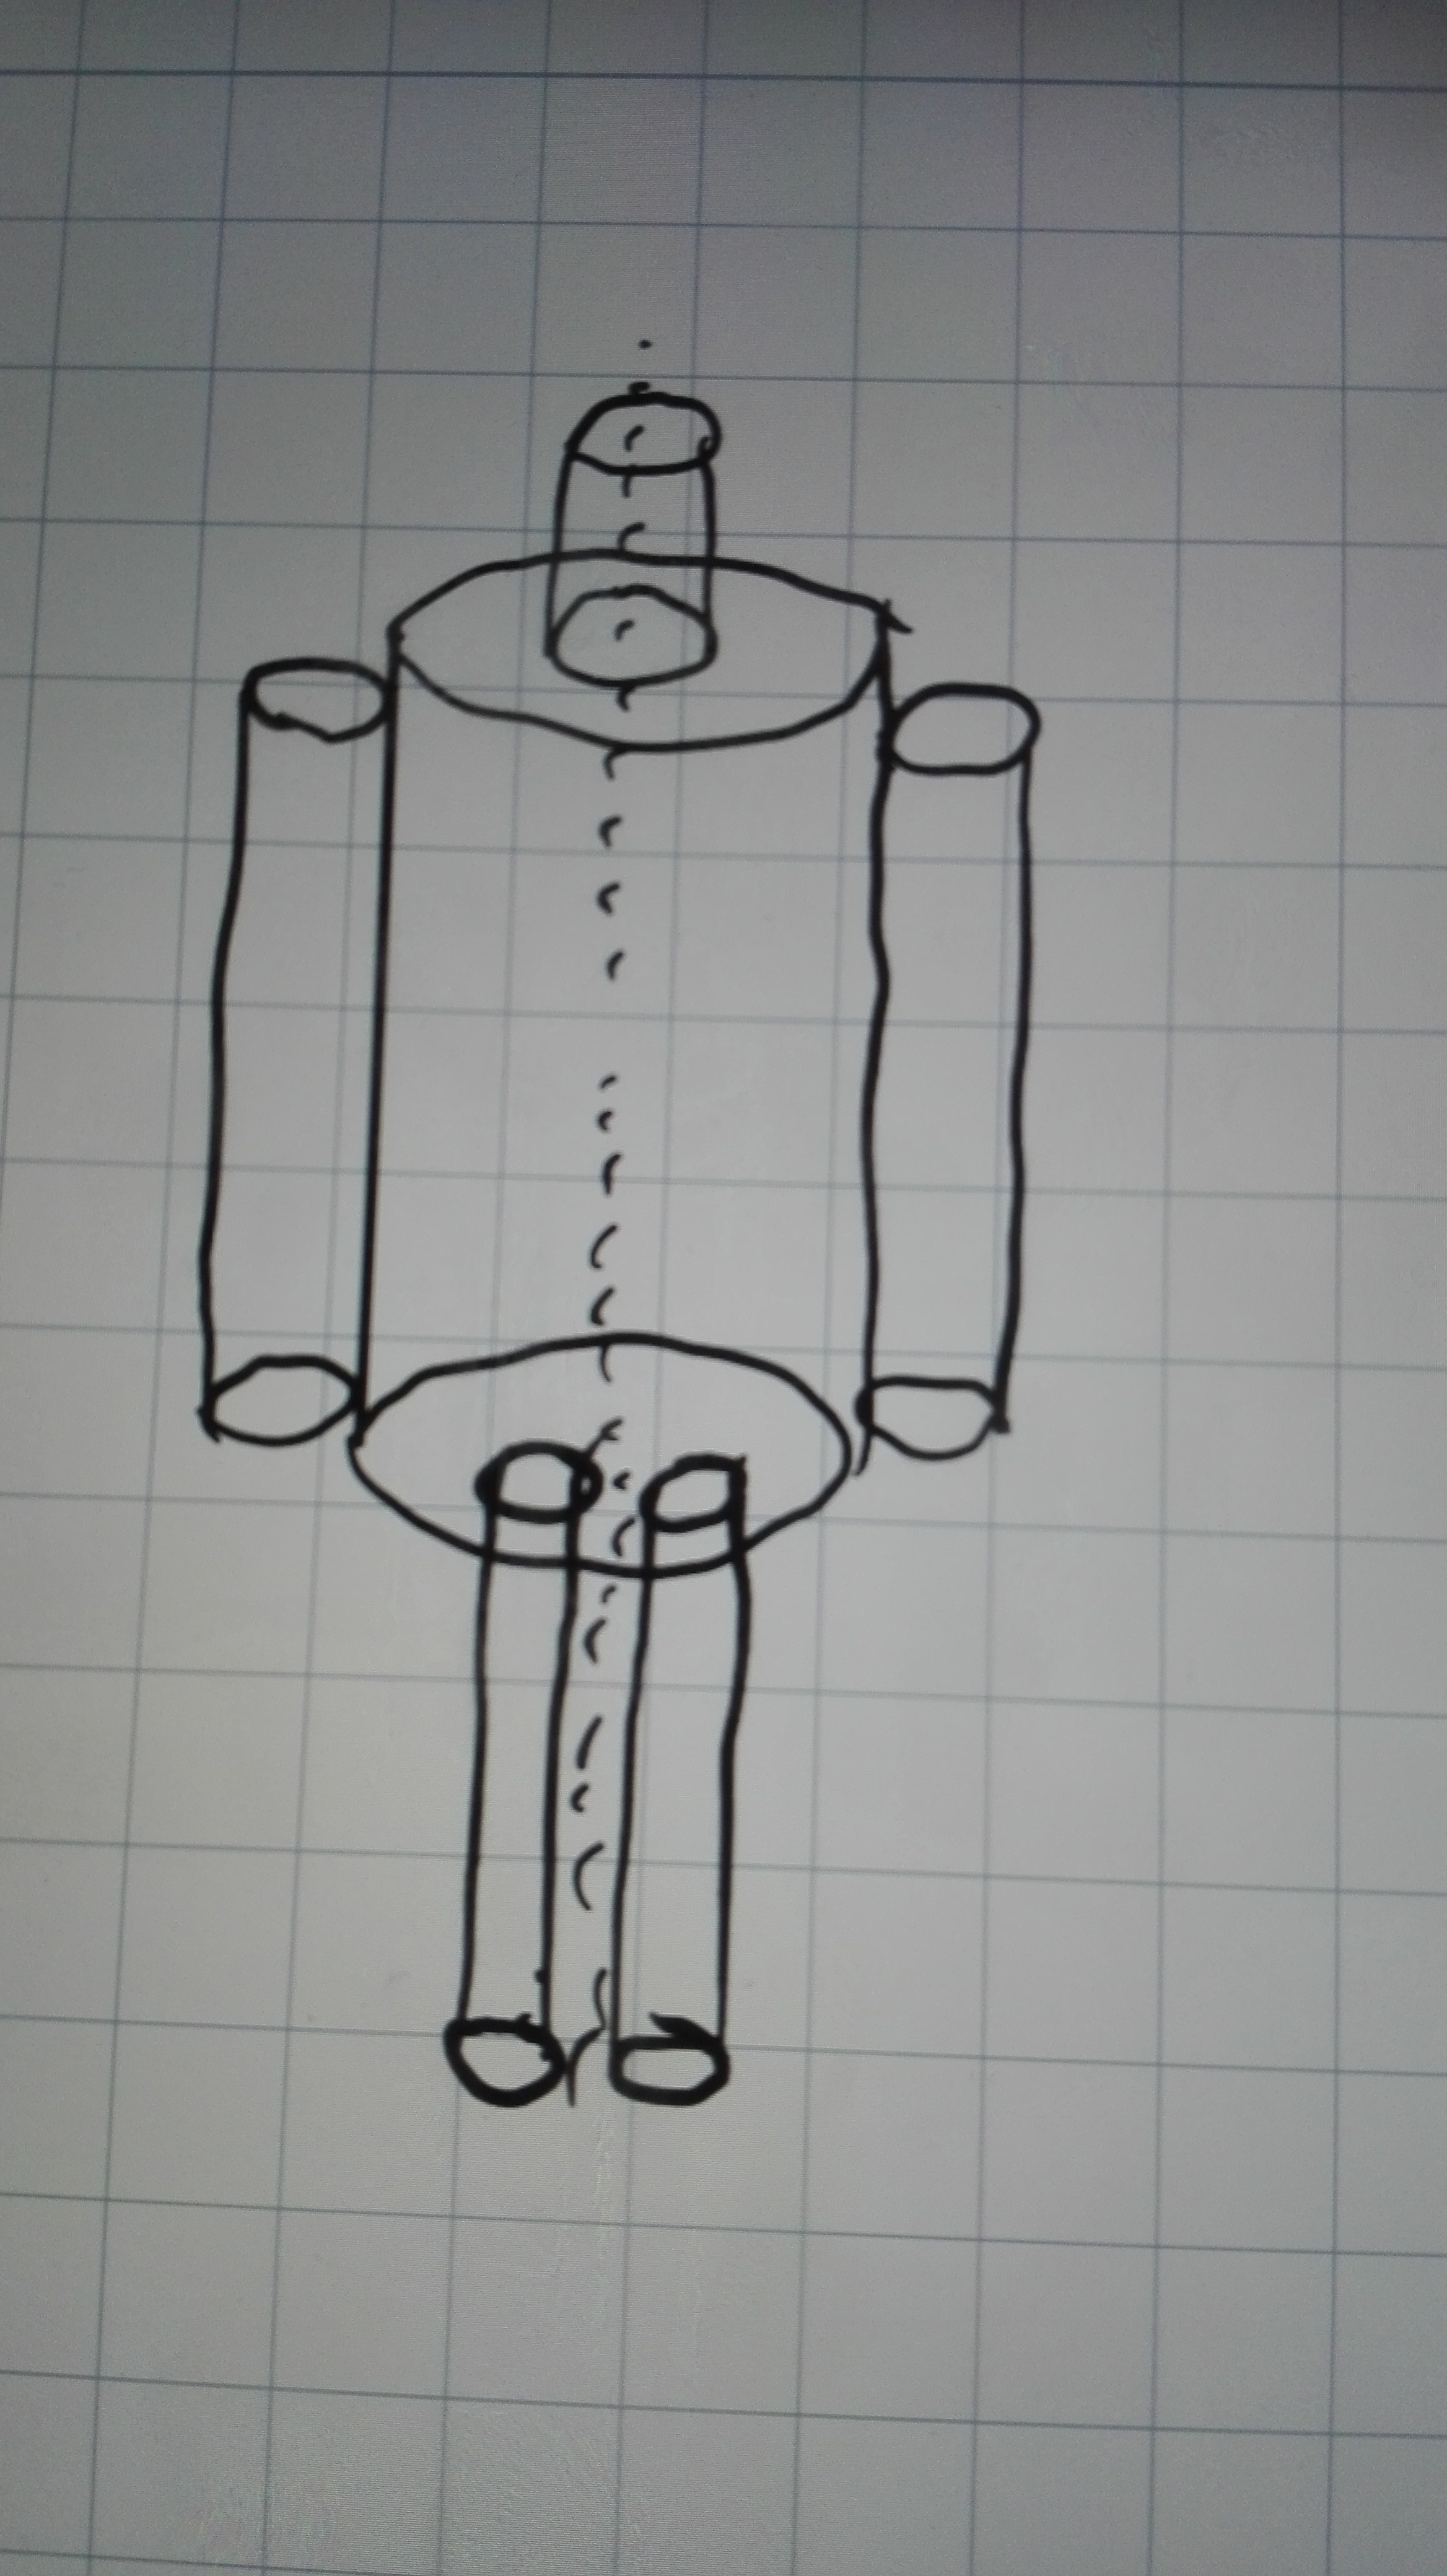
\includegraphics[width=\textwidth]{images/puppe_an.jpg}
\caption{Puppe mit angezogenen Armen (Pos. 1)}
\end{subfigure}
\begin{subfigure}{0.495\linewidth}
\centering
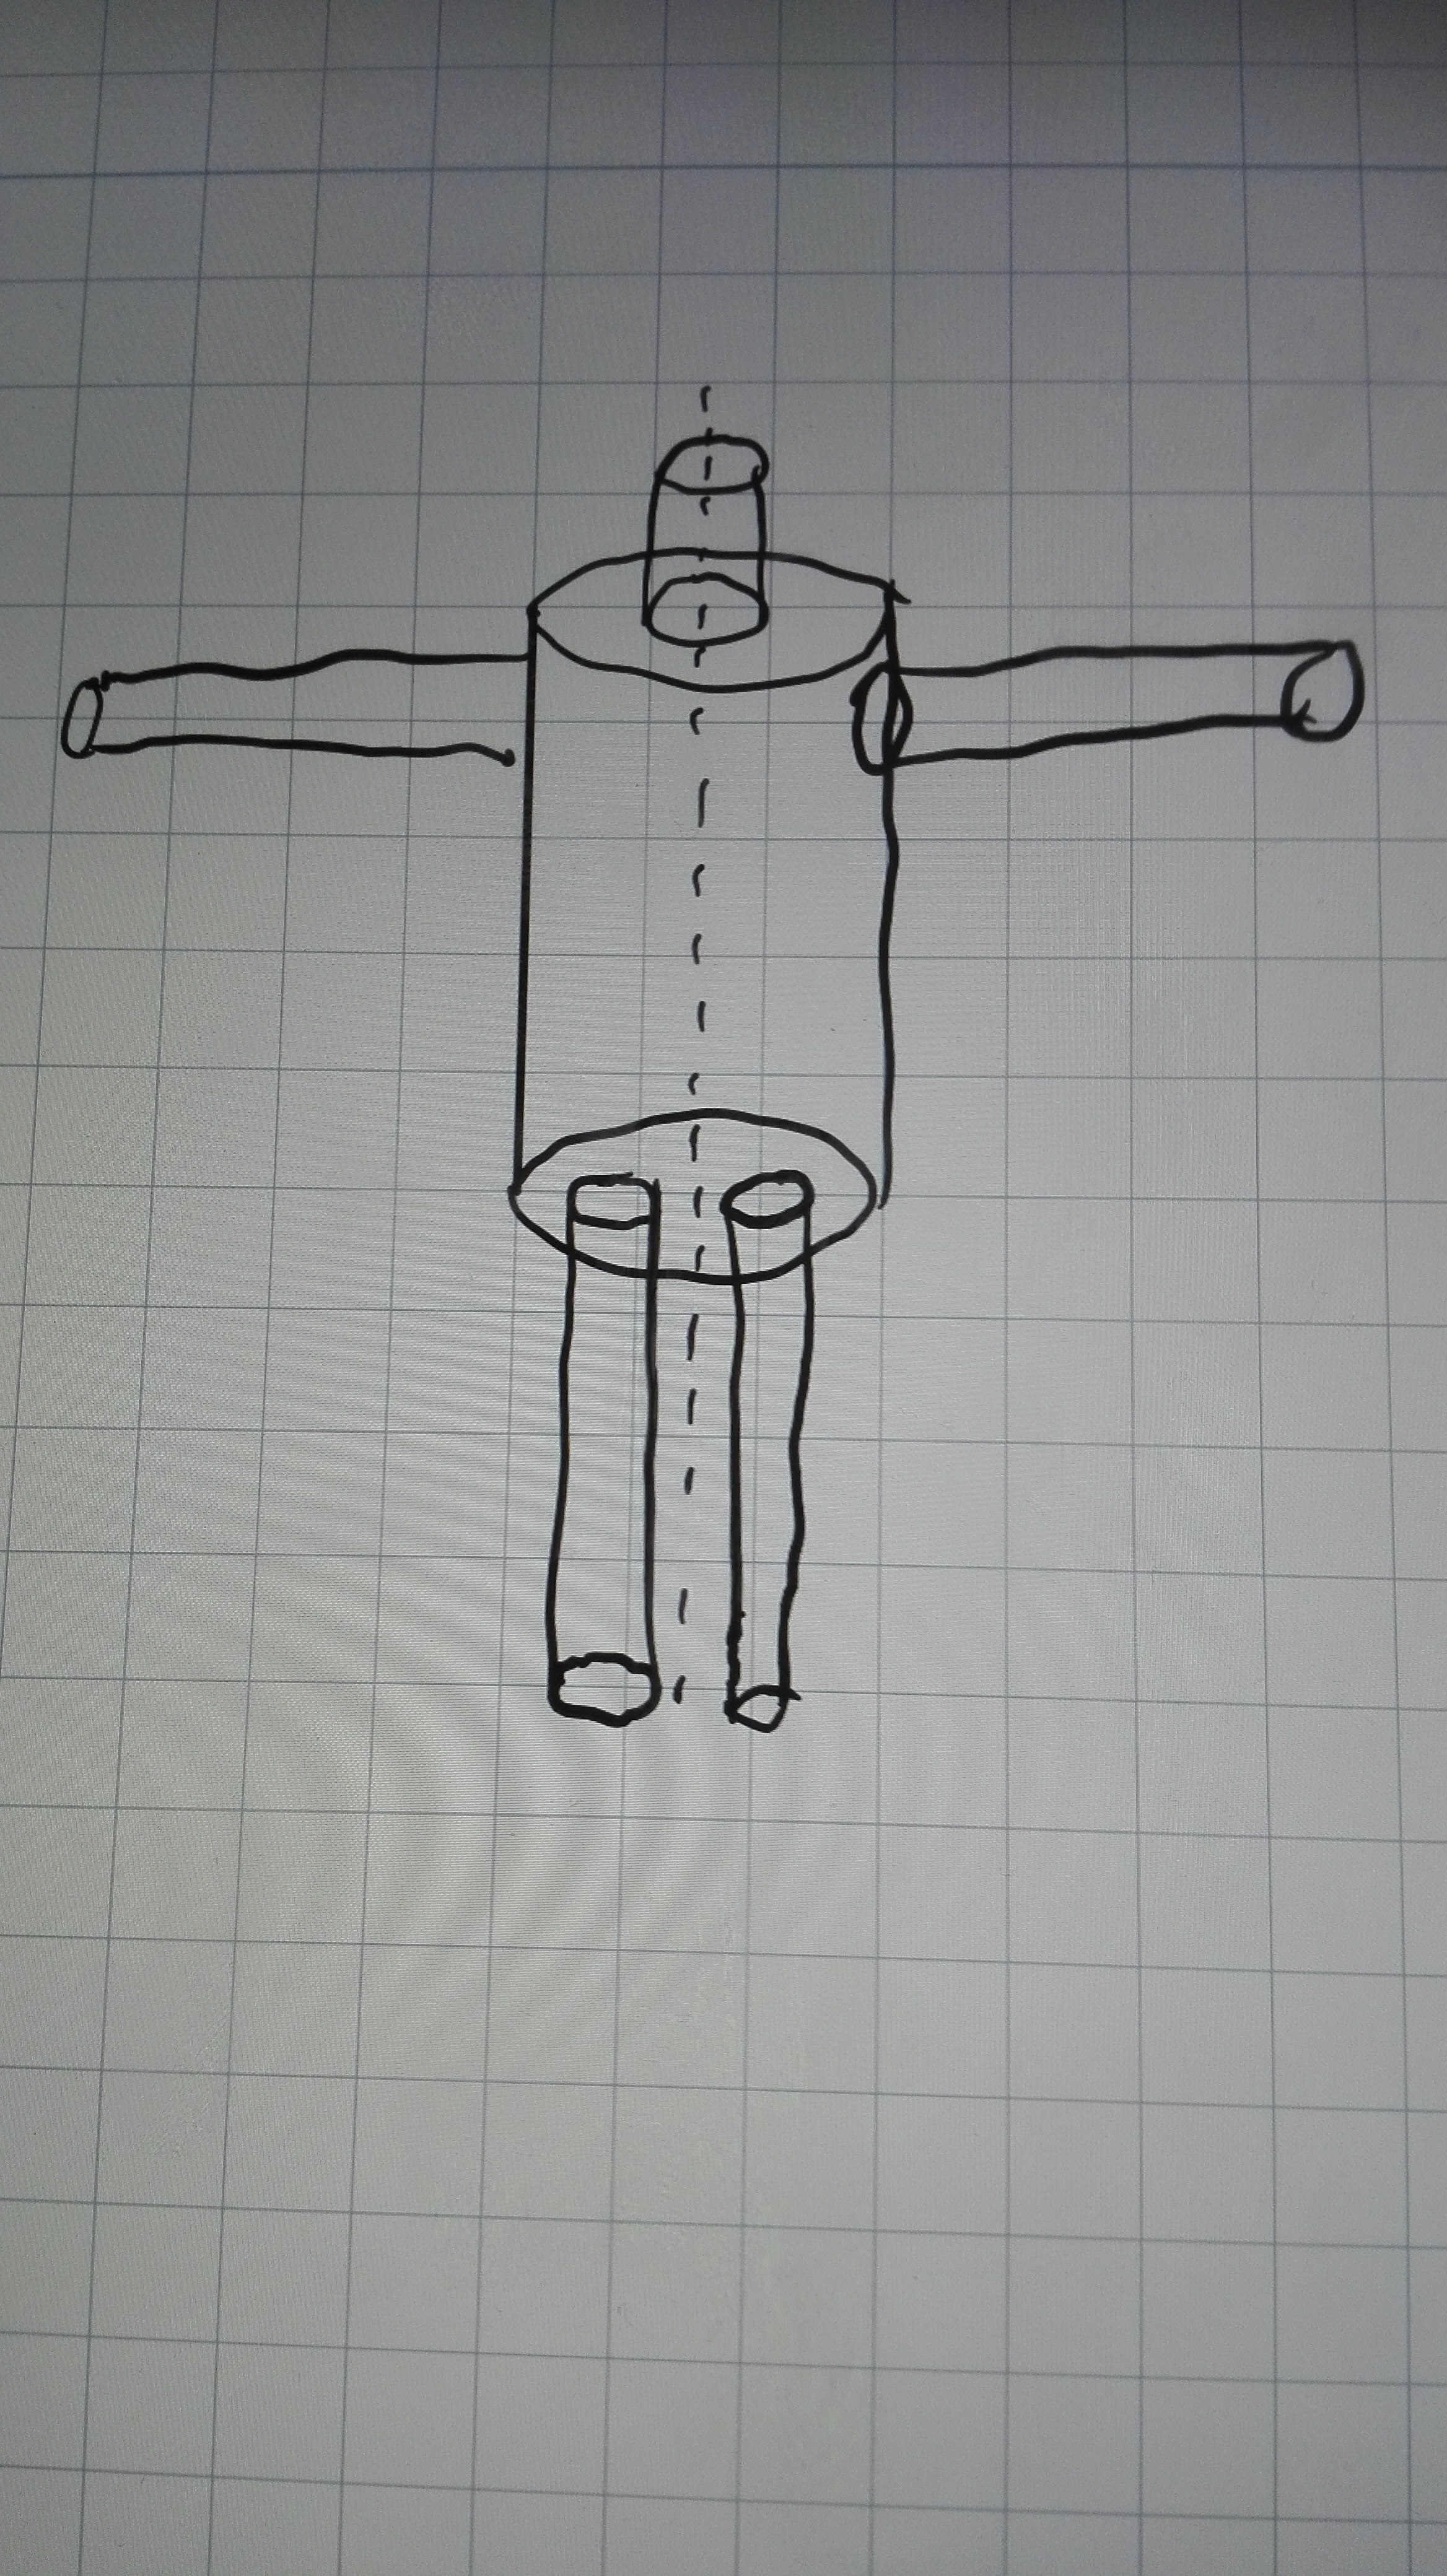
\includegraphics[width=\textwidth]{images/puppe_aus.jpg}
\caption{Puppe mit ausgestreckten Armen (Pos. 2)}
\end{subfigure}
\end{figure}

\flushleft{Die\;}\justifying Massen der einzelnen Zylinder wurden mithilfer der Formel $m= \rho \cdot V$ bestimmt und lauten wie folgt:

\begin{subequations}
\begin{align}
\text{Kopf: \input{m_Kopf.tex}}\label{eq:Kopf}\\
\text{Torso: \input{m_Torso.tex}}\label{eq:Torso}\\
\text{Arm: \input{m_Arm.tex}}\label{eq:Arm}\\
\text{Bein: \input{m_Bein.tex}}\label{eq:Bein}
\end{align}
\end{subequations}

\flushleft{$V$\;}\justifying stellt dabei die verschiedenen Zylindervolumen dar

\begin{subequations}
\begin{align}
 V_{\text{Kopf}} &= \input{V_Kopf.tex}\\
 V_{\text{Torso}} &= \input{V_Torso.tex}\\
 V_{\text{Arm1,2}} &= \input{V_Arm.tex}\\
 V_{\text{Bein1,2}} &= \input{V_Bein.tex},
\end{align}
\end{subequations}

\flushleft{während\;}\justifying $\rho$ die Dichte von Buchenholz darstellt \cite{Holzdichte}:
\begin{align}
    \rho = \SI{760}{\kilo\gram\meter\tothe{-3}}.
\end{align}

\subsubsection{Puppe Position 1} % Puppe 1 ---------------------------------------------------------------------------------------------------------

\flushleft{Um\;}\justifying das experimentelle Trägheitsmoment der Puppe in Position 1 berechnen zu können, werden die die Trägheitsmomente der
einzelnen Zylinder mit der Formel \eqref{eq:18} und den Werten aus Tabelle \ref{tab:3} bestimmt. Die individuellen Trägheitsmomente werden
aufsummiert um das Trägheitsmoment der Puppe für die einzelnen Periodendauern zu erhalten. Abschließend werden die Trägheitsmomente
mit der Mittelwertsformel \eqref{eq:10a} gemittelt um auf das Gesamtträgheitsmoment zu kommen: 
\begin{align}
\intertext{Demnach folgt aus der Summe der einzelnen $I_K$'s}
I_{K,sum.} &= \sum_{i=1}^{6} I_K
\intertext{und dem gebildeten Mittel der $I_{K,sum.}$'s das Trägheitsmoment der Puppe in Position 1:
}
\overline{I_{K,exp.}} &= \input{I_Puppe_an_exp_mean.tex}
\intertext{Bei dem theoretischen Trägheitsmoment der Puppe in Position 1 wird ähnlich verfahren. Die Trägheitsmomente der einzelnen Zylinder werden 
mit der Formel \eqref{eq:4} bestimmt und aufsummiert. Daraus folgt der theoretische Wert:
}
I_{K,lit.} &= \input{I_Puppe_an_theo.tex}
\intertext{Der relative Fehler des Trägheitsmoments der Puppe in Position 1 ist:
}
\frac{\overline{I_{K, exp.}} - I_{K, lit.}}{I_{K, lit.}} &= \input{RF_I_Puppe_an.tex}
\end{align}

\subsubsection{Puppe Position 2}\justifying % Puppe 2 ---------------------------------------------------------------------------------------------------------

\flushleft{Das\;}\justifying experimentelle Trägheitsmoment der Puppe in Position 2 ist:
\input{I_Puppe_aus_exp_mean.tex}

\flushleft{Das\;}\justifying theoretische Trägheitsmoment der Puppe in Position 2 ist:
\input{I_Puppe_aus_theo.tex}

\flushleft{Das\;}\justifying relative Fehler des Trägheitsmoments der Puppe in Position 2 ist:
\input{RF_I_Puppe_aus.tex}
\newpage
% Diskussion %%%%%%%%%%%%%%%%%%%%%%%%%%%%%%%%%%%%%%%%%%%%%%%%%%%%%%%%%%%%%%%%%%%%%%%%%%%%%%%%%%%%%%%%%%%%%%%%%%%%%%%%%%%%%%%%%%%%%%%%%%%%%%%%%%%%%%%%%%%
\section{Diskussion}\justifying
Nach der Auswertung folgt nun eine kurze Diskussion der berechneten Werte.\\
Die Winkelrichtgröße D \eqref{eq:17} scheint in einer passenden
Größenordnung vorzuliegen, allerdings lässt sich anhand der Formel \eqref{eq:16}
und der Tabelle \ref{tab:2} ein Fehler in der Messung in der Messung erkennen.
Da die Winkelrichtgröße grundsätzlich konstant sein sollte, ergibt sich bei einem
doppelt so großen Winkel eine doppelt so große Kraft. Dies ist hier nicht unbedingt der Fall
wie die Werte für \SI{90}{\degree} und \SI{180}{\degree} zeigen. Diese Messungenauigkeit
ergibt sich aus dem Problem des Nullpunkts beim Newtonmeter. In der Messung wurde das
Newtonmeter an die audgelenkte Stange gehalten, welche danach losgelassen wurde und die Kraft
anzeigte. Dabei kann es passieren, dass das Newtonmeter sich nicht perfekt am Stab
ansetzt und dann zu viel oder zu wenig ausgelenkt wird. Zudem ergibt sich eine gewisse
Ungenauigkeit beim Einstellen des Winkels. \\

\flushleft{Für}\justifying \;das Trägheitsmoment des Stabs wurde der Wert aus Formel \eqref{eq:15} bestimmt.
Bei dem Versuch wurde der Stab, auf dem sich die beiden Zylinder befanden, als masselos angenommen  und
die Zylinder als Punktmassen angenähert. Dabei wurde für die Auswertung bei der Periodendauer
nur die erste Nachkommastelle verwendet, da aufgrund der menschlichen Reaktionszeit sich
automatisch eine Ungenauigkeit für niedrigere Nachkommastellen ergibt.
Der Wert für das Trägheitsmoment $I_D$ wirkt dabei erstmal ziemlich klein, allerdings kann
dies täuschen, da eine theoretische Berechnung aufgrund der fehlenden Masse für den 
Drillstab nicht durcheführt werden konnte. Allerdings führen die Annäherungen in der 
Regel zu einer bestimmten Ungenauigkeit.
Der Graph \ref{fig:1} mit seinen Messwerten aus Tabelle \ref{tab:1} liegt dabei ohne große 
Abweichungen vor und spiegelt die in Formel \eqref{eq:11} gegebene Relation gut wieder.\\

\flushleft{Durch}\justifying \;die beiden Messungenauigkeiten in $D$ und $I_D$ ergeben
sich auch automatisch ein Fehler für die Trägheitsmomente der verschiedenen Körper.\\

\flushleft{Für\;} den Zylinder ergibt sich ein relaiver Fehler von $37\%$ und lässt sich
durch die bereits genannten Fehler erklären. \\
Für die Kugel ergibt sich ein relativer Fehler von $-34\%$ und kann wie beim Zylinder durch
die Messungenauigkeit in $D$ und $I_D$ begründet werden.
Allerdings zeigt sich, dass das Trägheitsmoment der Kugel kleiner als das Trägheitsmoment
des Zylinders ist. Dies erscheint aufgrund der gemessenen und berechneten Größen in Abschnitt \ref{sec:6.1}
sinnvoll. Beim Zylinder ist zu einen die Masse größer. Zum  anderen sind die Massepunkte weiter 
von der Rotationsachse entfernt als bei der Kugel.


\newpage

\printbibliography
\end{document}